\documentclass[12pt, a4paper]{article}

%%%%%%%%%%%%%%%%%%%%%%%%%%%%%%%%%%%%%% PACKAGES %%%%%%%%%%%%%%%%%%%%%%%%%%%%%%%%
\usepackage[swedish]{babel}
\usepackage[utf8]{inputenc}
\usepackage[hidelinks]{hyperref}
\usepackage{
  amsmath,
  amssymb,
  caption,
  color,
  float,
  graphicx,
  listings,
  siunitx,
  tikz,
  parskip,
  pdflscape,
  pgfgantt,
  scrextend,
}
\usepackage[
    backend=biber,
    style=ieee,
    sorting=none
]{biblatex}
\usepackage{csquotes}
\addbibresource{refs.bib}
\usetikzlibrary{positioning}

%%%%%%%%%%%%%%%%%%%%%%%%%%%%% LISTINGS SETTINGS %%%%%%%%%%%%%%%%%%%%%%%%%%%%%%%%

\definecolor{mygreen}{rgb}{0,0.4,0.1}
\definecolor{mygray}{rgb}{0.5,0.5,0.5}
\definecolor{mymauve}{rgb}{0.58,0,0.82}

\lstset{
  backgroundcolor=\color{white},   % choose the background color; you must add \usepackage{color} or \usepackage{xcolor}; should come as last argument
  basicstyle=\ttfamily,            % the size of the fonts that are used for the code
  breakatwhitespace=false,         % sets if automatic breaks should only happen at whitespace
  breaklines=true,                 % sets automatic line breaking
  captionpos=b,                    % sets the caption-position to bottom
  commentstyle=\color{mygreen},    % comment style
  deletekeywords={...},            % if you want to delete keywords from the given language
  escapeinside={\%*}{*)},          % if you want to add LaTeX within your code
  extendedchars=true,              % lets you use non-ASCII characters; for 8-bits encodings only, does not work with UTF-8
  firstnumber=1,                   % start line enumeration with line 1000
  frame=single,                    % adds a frame around the code
  keepspaces=true,                 % keeps spaces in text, useful for keeping indentation of code (possibly needs columns=flexible)
  keywordstyle=\color{blue},       % keyword style
  language=c,                      % the language of the code
  morekeywords={*,...},            % if you want to add more keywords to the set
  numbers=none,                    % where to put the line-numbers; possible values are (none, left, right)
  numbersep=5pt,                   % how far the line-numbers are from the code
  numberstyle=\tiny\color{mygray}, % the style that is used for the line-numbers
  rulecolor=\color{black},         % if not set, the frame-color may be changed on line-breaks within not-black text (e.g. comments (green here))
  showspaces=false,                % show spaces everywhere adding particular underscores; it overrides 'showstringspaces'
  showstringspaces=false,          % underline spaces within strings only
  showtabs=false,                  % show tabs within strings adding particular underscores
  stepnumber=2,                    % the step between two line-numbers. If it's 1, each line will be numbered
  stringstyle=\color{mymauve},     % string literal style
  tabsize=2,                       % sets default tabsize to 2 spaces
  title=\lstname                   % show the filename of files included with \lstinputlisting; also try caption instead of title
}

% FIX LISTINGS ENCODING PROBLEM
\lstset{literate=
  {á}{{\'a}}1 {é}{{\'e}}1 {í}{{\'i}}1 {ó}{{\'o}}1 {ú}{{\'u}}1
  {Á}{{\'A}}1 {É}{{\'E}}1 {Í}{{\'I}}1 {Ó}{{\'O}}1 {Ú}{{\'U}}1
  {à}{{\`a}}1 {è}{{\`e}}1 {ì}{{\`i}}1 {ò}{{\`o}}1 {ù}{{\`u}}1
  {À}{{\`A}}1 {È}{{\`E}}1 {Ì}{{\`I}}1 {Ò}{{\`O}}1 {Ù}{{\`U}}1
  {ä}{{\"a}}1 {ë}{{\"e}}1 {ï}{{\"i}}1 {ö}{{\"o}}1 {ü}{{\"u}}1
  {Ä}{{\"A}}1 {Ë}{{\"E}}1 {Ï}{{\"I}}1 {Ö}{{\"O}}1 {Ü}{{\"U}}1
  {â}{{\^a}}1 {ê}{{\^e}}1 {î}{{\^i}}1 {ô}{{\^o}}1 {û}{{\^u}}1
  {Â}{{\^A}}1 {Ê}{{\^E}}1 {Î}{{\^I}}1 {Ô}{{\^O}}1 {Û}{{\^U}}1
  {ã}{{\~a}}1 {ẽ}{{\~e}}1 {ĩ}{{\~i}}1 {õ}{{\~o}}1 {ũ}{{\~u}}1
  {Ã}{{\~A}}1 {Ẽ}{{\~E}}1 {Ĩ}{{\~I}}1 {Õ}{{\~O}}1 {Ũ}{{\~U}}1
  {œ}{{\oe}}1 {Œ}{{\OE}}1 {æ}{{\ae}}1 {Æ}{{\AE}}1 {ß}{{\ss}}1
  {ű}{{\H{u}}}1 {Ű}{{\H{U}}}1 {ő}{{\H{o}}}1 {Ő}{{\H{O}}}1
  {ç}{{\c c}}1 {Ç}{{\c C}}1 {ø}{{\o}}1 {å}{{\r a}}1 {Å}{{\r A}}1
  {€}{{\euro}}1 {£}{{\pounds}}1 {«}{{\guillemotleft}}1
  {»}{{\guillemotright}}1 {ñ}{{\~n}}1 {Ñ}{{\~N}}1 {¿}{{?`}}1 {¡}{{!`}}1
}

%%%%%%%%%%%%%%%%%%%%%%%%%%%%%%%  NICE PALETTE  %%%%%%%%%%%%%%%%%%%%%%%%%%%%%%%%%

% https://images.squarespace-cdn.com/content/v1/638773c92dfb4812d5f5ff28/1669823793535-UWL204TLLHME6SFDP2QZ/image-asset.png
\definecolor{navy}{RGB}{16,37,38}
\definecolor{ginger}{RGB}{205,126,89}
\definecolor{seafoam}{RGB}{69,115,115}
\definecolor{sunflower}{RGB}{221,178,71}
\definecolor{jean}{RGB}{90,104,104}


%%%%%%%%%%%%%%%%%%%%%%%%%%%%%%%%%  COVER PAGE %%%%%%%%%%%%%%%%%%%%%%%%%%%%%%%%%

%%%%%%%%%%%%%%%%%%%%%%%%%%%%%%%%%  TITLE PAGE  %%%%%%%%%%%%%%%%%%%%%%%%%%%%%%%%%

%\title{Projektrapport - Binäranalys med en hybrid av automatiska och manuella metoder}
%\author{
%    Loke Gustafsson \and
%    Samuel Kyletoft \and
%    Enayatullah Norozi \and
%    Albin Otterhäll \and
%    Clara Salberg \and
%    Linus Wallman
%}
%\date{2023-02-20}

%%%%%%%%%%%%%%%%%%%%%%%%%%%%%%%%%% COMMANDS %%%%%%%%%%%%%%%%%%%%%%%%%%%%%%%%%%%%
\newcommand{\stoe}{S$^2$E}

%%%%%%%%%%%%%%%%%%%%%%%%%%%%% DOCUMENT STRUCTURE %%%%%%%%%%%%%%%%%%%%%%%%%%%%%%%

\begin{document}

%%% Cover image %%%
\vtop{
    \null\vspace{-25mm}
    \centerline{
\includegraphics[width=1\textwidth]{figures/chalmers_gu_logo.jpg}}
    \vspace{0.5mm}
    \rule{\textwidth}{1pt}
}

%%% Cover text %%%
\mbox{}
\vfill
\textbf{{\Huge Binäranalys med en hybrid av automatiska och manuella metoder}} \\[0.5cm]
Bachelor of Science Thesis in Computer Science and Engineering \setlength{\parskip}{1cm}

\noindent
{\Large Loke Gustafsson, Samuel Kyletoft, Enayatullah Norozi, Albin Otterhäll,
Clara Salberg, Linus Wallman} \setlength{\parskip}{1.5cm}

%%% Cover footer %%%

\rule{\textwidth}{1pt}
\textsc{Chalmers University of Technology} \\
\textsc{University of Gothenburg} \\
{\small Department of Computer Science and Engineering} \\
{\small Gothenburg, Sweden \the\year \\


\newpage
% TITLE PAGE
\newpage
\thispagestyle{empty}
\begin{center}

	\textbf{\Large \ambaTitle} \\[1cm]

    {\linespread{1.2}\large
        \StrSubstitute{\ambaAuthors}{,}{\\}
        \\
    }
	
	\vfill 	

	\ambaDepartment \\
	\textsc{Chalmers University of Technology} \\
	\textsc{University of Gothenburg} \\
	\ambaCityCountryYear
\end{center}


\newpage
%\thispagestyle{plain}
%\vspace*{4.5cm}
{The authors grant to Chalmers University of Technology and University of Gothenburg the
non-exclusive right to publish the work electronically and in a non-commercial purpose make it
accessible on the Internet. The authors warrant that they are the authors to the work, and
warrant that the work does not contain text, pictures or other material that violates
copyright law.
The authors shall, when transferring the rights of the work to a third party (for example a
publisher or a company), acknowledge the third party about this agreement. If the authors have
signed a copyright agreement with a third party regarding the work, the authors warrant
hereby that they have obtained any necessary permission from this third party to let Chalmers
University of Technology and University of Gothenburg store the work electronically and make
it accessible on the Internet.}

Supervisor: Iulia Bastys \\
Examiner: Joachim von Hacht \setlength{\parskip}{1cm}

Chalmers University of Technology\\
University of Gothenburg\\
\ambaDepartment \\
SE-412 96 Gothenburg\\
Telephone +46 31 772 1000 \setlength{\parskip}{0.5cm}

\vfill
\ambaCityCountryYear


%\maketitle

\newpage

\tableofcontents
\newpage

\addcontentsline{toc}{section}{Begreppslista}
\section*{Begreppslista}
\begin{labeling}{begreppslista}

    \item [\textbf{Assembler}] Assembler (jfr.\ eng.\ \emph{assembly}) är ett
    lågnivåspråk som direkt kan översättas till maskinkod.

    \item[\textbf{Basic block}] \emph{Basic block} (jfr.\ sv.\ grundblock) är en
    sekvens av instruktioner som saknar hopp eller förgreningar bortsett från
    början och slutet av blocket. Är oftast expanderade till att bli så långa
    som möjligt

    \item [\textbf{Black-box analys}] Black-box analys (jfr.\ sv.\
    svartlådeanalys) är en analys av ett objekt som endast betraktar dess
    yttre utseende och beteende, till skillnad från white-box-analys som även
    betraktar vad som händer inuti.

    \item [\textbf{Binär}] En binär (jfr.\ eng.\ \emph{binary}) är en fil som
    innehåller ett programs maskinkod och data.

    \item [\textbf{Återanropsfunktion}] Återanropsfunktion (jfr.\ eng.\
    \emph{callback function}) är funktioner som läggs i en \emph{hook} (jfr.\ sv.\ krok) för
    att exekveras vid ett visst tillstånd.

    \item [\textbf{CTF}] CTF (\emph{Capture the Flag}, jfr.\ sv.\ fånga
    flaggan) är i datorsäkerhetssammanhang är en utmaning eller övning i att
    hitta gömda ''flaggor'' i program med avsiktliga säkerhetshål.

    \item [\textbf{Dynamisk analys}] Dynamisk analys (jfr.\ eng.\ \emph{dynamic
        analysis}) är när en binär analyserar genom att exevera binären i en
    kontrollerad miljö för att i detalj registrera vad binären gör.

    \item [\textbf{ELF}] ELF (\emph{Executable and Linkable Format}, jfr.\ sv.\
    exekverbart och länkbart format). Filformatet för exekverbara filer
    på Linux och liknande system. Innehåller maskinkod och länkar till andra
    ELF-filer.

    \item [\textbf{Exekveringsmotor}] En exekveringsmotor (jfr.\ eng.
    \ \emph{execution engine}) är ett program som exekverar ett programs
    instruktioner.

    \item [\textbf{Fuzztestning}] Fuzztestning (jfr.\ eng.\ \emph{fuzz testing})
    är att slumpmässigt generera indata till ett system i ett försök att hitta
    buggar eller genom frånvaron av dåligt beteende betryggas i systemets
    kvalité. Vissa fuzztestmotorer genererar ny indata med genetiska algoritmer
    och vissa använder \emph{white-box} binärinstrumentation för att evaluera indata.

    \item [\textbf{Grey-box analysis}] \emph{Grey-box analysis} (jfr.\ sv.\
    \emph{grålådeanalys}) är en teknik som kombinerar \emph{black-box} och \emph{white-
        box} för att bilda en bredare analys. Ett användingsområde kan vara där
    dokumentationen är begränsad om ett programs interna struktur.

    \item [\textbf{Heap}] Heapen är ett område i minne som samtliga trådar i
    en process har tillgång till. Används för objekt som man inte vet storleken på
    innan man exekverar programmet; samt objekt som ska delas mellan en process
    trådar.

    \item [\textbf{Heuristik}] Heuristik är en praktisk metod för att lösa
    problem baserat på tidigare erfarenhet. En metod som är inte är fullständig
    utan baserad på tumregel.

    \item [\textbf{Hook}] \emph{Hook} (jfr.\ sv.\ krok) är en lista på återanropsfunktioner
    som ska köras vid ett specifikt tillstånd.

    \item [\textbf{Instrumentering}] Instrumentering (jfr.\ eng.\
    \emph{instrumentation}) är mätning av ett programs prestanda. Används för
    att hitta buggar och hitta kontrollflöden.

    \item [\textbf{IPC}] IPC (\emph{Inter-process communication}, jfr.\ sv.\
    interprocesskommunikation) är ett samlingsbegrepp för olika tekniker
    för att trådar i olika processer att kommunicera med varandra.

    \item [\textbf{KLEE}] KLEE är den symboliska exekveringsmotorn som används
    av \stoe{}.

    \item [\textbf{Maskinkod}] Maskinkod (jfr.\ eng.\ \emph{machine code}) är
    digital kod som CPU:n kan tolka och arbeta med.

    \item [\textbf{Tillståndssammanslagning}] Tillståndssammanslagning (jfr.\
    eng.\ \emph{state merging}) möjliggör att antingen automatiskt eller
    manuellt slå ihop olika stigar mellan tillstånd. Används för att öka
    presdandan.

    \item [\textbf{Systemanrop}] Systemanrop (jfr.\ eng.\ \emph{syscall}) är
    mjukvaruavbrott som program använder för att kunna anropa
    operativsystemskärnan på ett sätt som liknar funktionsanrop.

    \item [\textbf{Pekare}] Pekare (jfr.\ eng.\ \emph{pointer}) är en minnesadress som
    vanligtvis pekar på ett värde på stacken eller heapen.

    \item [\textbf{Process}] En process är en
    operativsystemabstraktion som speciellt innehåller en memory
    map(jfr.\ sv.\ minneskarta) tillsammans med ett antal trådar och
    andra operativsystemsresurser såsom fildeskriptorer (jfr.\
    eng.\ \emph{File descriptor}).

    \item [\textbf{QEMU}] QEMU (\emph{Quick Emulator}, jfr.\ sv.\ snabb
    emulator) är ett välunderhållet öppen källkods emulatorramverk
    med stöd för många plattformar och som stöder både \emph{user-space}
    emulering av en process samt emulering av ett helt system.

    \item [\textbf{Utpressningsprogram}] Utpressningsprogram (jfr.\ eng.\
    \emph{ransomware}) är en sorts skadeprogram som syftar till att göra ett it-
    system oanvändbar genom kryptering av data som endast kan avkrypteras med
    en nyckel.

    \item [\textbf{RCE}] RCE (\emph{Remote code execution}, jfr.\ sv.
    \ fjärrkodsexekvering) är en sårbarhet som tillåter körning av
    godtyckliga kommandon eller kod på en måldator.

    \item [\textbf{Reverse Engineering}] \emph{Reverse engineering} (jfr.\ sv.\
    demontering eller backlängeskonstruktion) är en process där man från en
    befintlig artefakt försöker återskapa källkodsinstruktionerna
    skrivna av de ursprungliga utvecklarna av artefakten.

    \item [\textbf{Runtime}] \emph{Runtime} (jfr.\ sv.\ körtid) är tidsspannet
    från det att ett program börjar exekveras, tills dess att programmet har
    slutat att exekveras.

    \item [\textbf{\stoe}] \stoe (\emph{The Selective Symbolic Execution
        Platform}, jfr.\ sv.\ Den selektiva exekveringsplattformen) är
    en platform som tillhandahåller symbolisk exekvering inuti den virtuella
    maskinen QEMU.\@

    \item [\textbf{SMT-lösare}] SMT-lösare (jfr.\ eng.\ \emph{Satisfiability Modulo
        Theories solver}) är ett program som kan lösa
    ekvationssystem för olika matematiska objekt. Exempel på
    teorier är modulär aritmetik eller bitvektorer. En SMT-lösare
    kan till exempel lösa ekvationer konstruerade i symbolisk
    exekvering.

    \item [\textbf{Stack}] Område i minnet som reserveras för varje
    enskild tråd. På stacken förvaras värden där man redan vid
    kompilering känner till värdets minnesstorlek.

    \item [\textbf{Starkt anslutna komponenter}] Starkt anslutna komponenter
    (jfr.\ eng.\ \emph{Strongly Connected Components}) är en riktad delgraf där
    varje nod har en väg sådant att det går att nå alla andra noder i delgrafen.

    \item [\textbf{Statisk analys}] Statisk analys (jfr.\ eng.\ \emph{static
        analysis}) är binäranalys där man endast utifrån maskinkoden på disk
    försöker dra slutsater om binärens beteende.

    \item [\textbf{Symbolisk exekvering}] Symbolisk exekvering (jfr.\ eng.\
    \emph{symbolic execution}) är att tilldela variabler symboliska, i motsats
    till konkreta värden under programmets exekvering. Med denna analysteknik
    kan enskilda körningar ge information som annars hade krävt en uttömmande
    sökning.

    \item [\textbf{Symbolisk fuzzing}] Symbolic fuzzing (jfr.\ eng.
    \ \emph{symbolic fuzz testing}) är en teknik som kombinerar symbolisk
    exekvering och fuzzingtestning. Kombinationen bevarar kodstrukturen och kan
    samtidigt lösa komplexa symboliska restriktioner.

    \item [\textbf{Symbolisk operation}] Symbolisk operation (jfr.\ eng.\ \emph{symbolic
        operation}) är operationer med symboliska värden.

    \item [\textbf{Tråd}] Thread (jfr.\ eng.\ \emph{thread}) är en av flera
    parallella instruktionssekvenser inom en process.

    \item [\textbf{White-box analysis}] \emph{White-box analysis} (jfr.\ sv.
    \ vitlådsanalys) är en analysmetod som behandlar en applikations
    interna struktur i kontrast till black-box analys som enbart betraktar
    funktionaliteten.

\end{labeling}


\newpage

\section{Inledning}
Attacker mot organisationers eller nationers IT-system har ofta förrödande
direkta och indirekta konsekvenser för de drabbade. Enligt företaget Cybereason
svarade över 70 procent av de över 1400 tillfrågade säkerhetsspecialister i en
av deras studier att deras organisation hade utsats för
\emph{Utpresningsprogram} (engelska: \emph{ransomware}) minst en gång de senaste
24 månaderna \cite{cyberreason2021, cyberreason2022}. Cybereasons rapporter
beskriver att några av de direkta följderna av att en lyckad attack är höga
kostnader för organisationen; stoppad produktion; konsekvenser från reglerare;
och skadat anseende. Enligt Cybereasons rapporter leder de höga kostnaderna till
bland annat uppsägningar av anställda för att kunna kompensera. I en artikel i
Bloomberg Newsweek \cite{gallagher2023} beskrivs hur cancerpatienter som behövde
akut sjukvård förflyttades till sjukhus med fungerade datorsystem när Irlands
offentliga sjukhussystem låg nere. \cite{hse_report} Ransomware attacker
möjliggörs tack vare säkerhetsbrister i programvarorna som finns på offrens
datorsystem.

Flertalet arbeten existerar inom domänen binäranalys och dess analystekniker. Fowze \cite{fowze_mem_vul}
beskriver verkyget \emph{SEESAW}, ett verktyg för att analysera
minnessårbarheter i protokollstacken. Fokuset ligger på att undersöka USB och
blåtandsmoduler med hjälp av en hybrid av analysmetoder: statisk analys och
dynamisk analys. \emph{SEESAW} implementerar en algoritm som tillämpar
bidirektionell kommunikation mellan en statisk analys som tillhandahåller ett
mål i binären till en riktad symbolisk exekvering dvs den dynamiska analysen som
ger tillbaka en bestämd funktionspekare för att komplettera och öka precisionen
av analysen.  

Ett annat verktyg för binäranalys är X-Force som utför exekvering av binära 
filer utan input eller miljö och utforskar vägar programmet kan ta genom att 
tvinga exekvering av förgreningar\cite{xforce}. X-force kan skapa en graf över 
programmets kontrollflöde och visa beteenden även om de har gömts genom
obfuskering.

%Detta projekt ämnar utveckla ett binäranalysverktyg för generell reverse
%engineering, det vill säga en applikation vars uppgift är att analysera binära
%program utan kännedom om källkoden utifrån ett datorsäkerhetsperspektiv.

Projektet ämnar utveckla binäranalysverktyget AMBA för interaktiv visualisering
av symbolisk fuzzing som möjliggör utforskande binäranalys med hjälp av
symbolisk exekvering. Visualiseringen ska presenteras i ett grafiskt
användargränssnitt där användaren kan interaktivt följa exekveringen och
prioritera exekveringsvägar. Verktyget ämnar att, genom mänskligt fördelaktiga
representationer av programmets beteende, förbättra kommunikationen till
användaren och underlätta binäranalys inom skadeprogramsanalys och
sårbarhetsanalys.

Detta för att möjliggöra ett utforskande analysverktyg som kombinerar datorns
fördel i beräkningskraft och människans intuition. Symbolisk fuzzing löser
problemet av att inte behöva godtyckligt gissa input som leder till att en
specifik väg tas i ett program, och nyttan från människans intuition nyttjas på
samma sätt som med en dekompilator --- genom analys som leder till ökad
förståelse och insikt. Denna kombinationen gör det möjligt att på ett
användarvänligt sätt dra analytiska slutsatser om ett program i
maskinkodsformat och öka den abstrakta förståelsen av det och därmed underlätta
binäranalys baserad på symbolisk fuzzing.

\subsection{Avgränsningar}

Att skapa en en exekveringsmotor med stöd för bland annat symbolisk exekvering
skulle i praktiken innebära implementering av en emulator. Det är en relativ
stor och tidskrävande uppgift som dessutom kräver nogrann testning för att vara
korrekt och tillförlitlig. För att fastställa korrekthet ska applikationen
därför utnyttja existerande verktyg för att exekvera programmet med stöd för
symbolisk exekvering. Detta möjliggör också bredare plattformssupport jämfört
med en hemmasnickrad emulator.


\subsection{\Verktyg}

\stoe\cite{s2e} är en plattform för symbolisk exekvering som bygger på QEMU:s
virtuella maskin och använder KLEE\cite{klee}, en motor för symbolisk
exekvering, som interpreter för att möjliggöra symbolisk exekvering. \stoe\ är i
sin tur utbyggbart med möjlighet för användaren att skriva ett eget plugin för
att utföra analyser och används inom säkerhetsforskning för att till exempel
analysera skadlig kod. \stoe\ användes som del av Galactica-systemet som spelade
i DARPA Cyber Grand Challenge\cite{s2e_website}. \stoe\ är öppen källkod,
väldokumenterat och underhålls aktivt.

Ett alternativt verktyg för symbolisk exekvering är symQEMU\cite{symqemu},
som också kombinerar QEMU:s virtuella maskin med KLEE:s motor för symbolisk
exekvering. Till skillnad från \stoe\ kompilerar SymQEMU KLEE in i den
analyserade binären och har jämförelsevis hög prestanda. Däremot har SymQEMU
bristfällig dokumentation och är ej aktivt uppdaterat.

Då SymQEMU ej uppdateras aktivt och har bristfällig dokumentation kommer \stoe\
användas. Projektet avgränsas i och med att existerande verktyg (\stoe) kommer
användas istället för att bygga en motor för symbolisk exekvering från grunden.

\subsection{Begränsningar}

Att använda \stoe\ innebär att arbetet avgränsas till att, i praktiken, skapa
ett plugin som avlyssnar och styr motorn. Varken emulator eller motor ska
byggas och de uppgifter som ingår i att skapa en exekveringsmotor exkluderas.

Det innebär att fokus flyttas ifrån motorns tekniska detaljer till resterande
jobbet med att utveckla en användbar slutprodukt som bygger ut \stoe:s redan
existerande funktionalitet med ett grafiskt användargränsnitt och möjlighet att
stega igenom, analysera och interaktivt besluta om värden under exekvering.

Beslutet innebär också att applikationens utformning blir bunden till \stoe:s
tekniska begränsningar.



\subsection{Bakgrund}

Attacker mot organisationers eller nationers IT-system har ofta förrödande direkta och indirekt
konsekvenser för de drabbade. Enligt företaget Cybereason svarade över 70 procent av de över 1400
tillfrågade säkerhetsspecialister i en av deras studier att deras organisation hade utsats för
\emph{Utpresningsprogram} (engelska: \emph{ransomware}) minst en gång de senaste 24 månaderna.
\cite{cyberreason2021}\cite{cyberreason2022} Cybereasons rapporter beskriver att några av de
direkta följderna av att en lyckad attack är höga kostnader för organisationen; stoppad produktion;
konsekvenser från reglerare; skadat anseende. Enligt Cyberreaons rapporter leder de höga kostnaderna
till bland annat uppsägningar av anställda för att kunna kompensera. I en artikel i Bloomberg
Newsweek beskrivs hur cancerpatienter som behövde akut sjukvård förflyttades till sjukhus med
fungerade datorsystem när Irlands offentliga sjukhussystem låg nere.\cite{gallagher2023} I slutet
av 2021 överlämnade revisorfirman PWC deras granskningsrapport till HSE:s ledning där de går igenom.
\cite{hse_report} Ransomware attacker möjliggörs tack vare säkerhetsbrister i programvarorna som
finns på offrens datorsystem.

Under \emph{BlueHat} 2019 gav \emph{MSRC} (\emph{Microsoft Security Response Center}) en överblick
över Microsofts taktiker för hur de hanterar säkerhetsbrister i deras produkter och tjänster.
\cite{miller19} Taktikerna som listades var att
\begin{itemize}
	\item eliminera säkerhetsbristerna från början;
	\item implementera metoder för att försvåra utnyttjande av säkerhetsbrister;
	\item minimera platserna där attackerarna kan göra skada och förhindra åtkomst; samt slutligen
	\item minimera tidsfönstret då attackerare har tillgång till systemet med hjälp av aktiv övervakning.
\end{itemize}
Enligt Miller härstammar ungefär 70 procent av alla Microsofts CVEr från minnessäkerhetsbuggar. Om
hela klasser av säkerhetsbrister kan eliminieras genom att utveckla nya verktyg som underlättar för
utvecklare att finna dem kan man ha stor påverkan på antalet sårbarheter.

För att kunna hitta och undersöka minnessäkerhetsbuggar behöver man ibland betrakta maskinkod, med
anledningen att man vill
\begin{itemize}
  \item kunna kontrollera om det förekommer kompilatorbuggar som ger oväntad maskinkod i binären;
  \item se hur \emph{UB} (\emph{undefined behaviour}) har utnyttjats av kompilatorn; och
  \item enklare kunna börja analysera då man endast behöver en binär, och inte behöva integrera
djupt in i byggsystemet.
\end{itemize}

Det finns ett flertal metoder för att analysera en exekverbar binärer. Exempel på dessa är att: 
\begin{enumerate}
  \item disassemblera binären och läsa dess funktioner för att förstå vad de gör.
  \item dekompilera assemblykoden med ett verktyg som ger pseudokod, och sedan läsa denna mer
    läsbara koden.
  \item köra binären på speciella testfall och jämföra svaret med vad som förväntas. Om
    programmet implementerar en specifikation kan en existerande testsamling användas.
  \item fuzztesta binären, det vill säga automatiskt generera testfall tills ett orsakar en crash eller
    annat oönskat beteende i binären. Många fuzztestmotorer skapar testfall med en evolutionär
    algoritm, och många använder instrumentering över vilka programhopp som tas för att bedöma
    testfalls nyttighet.
  \item använda concolic testing, alltså fuzzing där en SMT solver genererar nya testfall genom att
    lösa för testfall som orsakar annorlunda programhopp.
  \item stega igenom programmet i en debugger för att se exakt vad programmet gör med viss input.
\end{enumerate}

Problematisk minneshantering har potential att påverka ett programs korrekthet och 
kan utnyttjas av fientliga aktörer i skadliga syften. Att minne hanteras på ett 
osäkert sätt är inte ovanligt, speciellt då proggrammet är skrivet i ett språk som är 
"memory unsafe" som exempelvis C/C++. Det är då lätt att vid utveckling av program 
göra misstag som introducerar sårbarheter, och kan vara svårare att upptäcka dessa 
sårbarheter när de väl introducerats, speciellt om det inkorrekta beteendet endast 
uppstår under körning med specifika indata.

Att läsa källkod är ett sätt att förstå program, men ibland är det gynnsamt att istället betrakta
maskinkoden direkt. Detta kan vara för att

Begreppet \textit{reverse engingeering} syftar på processen att söka insikt i hur en produkt 
(enhet/process/mjukvara/verktyg/system) arbetar, utan en etablerad insikt i dess interna 
uppbyggnad. Med andra ord syftar reverse engineering på att dekonstruera en produkt för att 
öka förståelsen av den. Detta görs genom att med olika metoder plocka isär produkten för 
att förstå hur den utför ett arbete. Reverse engineering är ett fundamentalt verktyg då insikt 
om en produkts design behövs men designspecifikationer ej existerar eller är tillgängliga. 
Reverse engineering har flera användningsområden, däribland då äldre produkter, vars design 
inte längre är tillgänglig, behöver undersökas, eller när funktionalitet försvunnit i 
utvecklingsaproccesen och behöver återfinnas. Reverse engineering är också användbart för 
att analysera fel som uppstår, för att förbättra delkomponenter eller för att diagnostisera 
en produkt.

För att bilda en allmän förståelse om ett program krävs både \textit{korrekt} och
\textit{abstrakt} förståelse. I detta avseende syftar \textit{korrekt} på
avsaknaden av felaktiga slutsatser och \textit{abstrakt} på möjligheten att
resonera om programmet generellt i motsats till att resonera om en specifik
konkret indata i taget.

% Metod 1-2, att läsa kod, kan ge en \textit{abstrakt} förståelse av vad
% programmet gör, men för att verifiera att huruvida resonemanget är korrekt krävs
% hypotestestning vilket kräver att programmet körs. Således går det inte att
% bilda en \textit{korrekt} förståelse genom att enbart läsa kod.

% Metod 3-5, att köra programmet på testfall, ger framförallt en
% black-box-förståelse av programmet. Tillgången till binären och
% exekveringsmiljön används endast som ett verktyg för att generera nya testfall.
% Fuzzing och concolic testing kan köras helautomatiskt och är \textit{korrekta}.
% Men ofta är en tillräckligt täckande sökning av indatarummet omöjlig, och då kan
% den automatiska analysen ha missat ett kvalitativt annorlunda beteende. Dessutom
% ger en omfattande uppsättning indata-utdata-par inte användaren samma
% information som källkoden ger. Därmed är helautomatiska analysmetoder inte
% \textit{abstrakta}. Notera att det inte nödvändigtvis tyder på en brist i den
% automatiska analysen att ett kvalitativt annorlunda beteende missas, för det
% gömda beteendet skulle kunna vara en konsekvens av komplicerad kod, som till
% exempel ett hoppvilkor beroende på en kryptografisk hash av indatan. Men en
% analysmetod borde kunna peka ut var dess förståelse tar slut, snarare än att
% utelämna detta fullständigt vilket är vad avsaknaden av testfall visar sig som.

% Med metod 6, en debugger, kan användaren följa exekveringen för en viss indata
% utan att riskera att missförstå hur datan transformeras. Om användaren har ett
% oändligt tålamod kan de göra detta om och om igen för olika indata genererade
% med till exempel fuzzing. Varje genomstegning ger information om koden som
% behandlar indatan men också viss information om övrig kod -- till exempel kan
% ett svårtaget hopp indikera en plats för användaren att rikta sin uppmärksamhet
% mot. Detta ger en både \textit{korrekt} och \textit{abstrakt} förståelse, men
% med en orimlig manuell arbetsbörda för användaren.

En helautomatisk \textit{korrekt} metod kan ge en \textit{abstrakt} förståelse
om processens förlopp visualiseras för användaren. Valet mellan manuell
arbetsbörda som ger djup förståelse och en testfallsgenerationsdriven process
som ger översiktlig förståelse kan genomföras av användaren om verktygen stödjer
hela spektrummet.

För att klargöra distinktionen mellan manuell och automatiska metoder för
binäranalys används följande use cases:

\begin{lstlisting}[
    label={list:first},
    language=Python,
    caption=Use case manuella metoder,
    frame=single
    ]
# Givet sträng-input från stdin
s = input()
if sha256(s) = "välkänd hash":
  print("Winner winner chicken dinner")
else:
  print("you lose")

\end{lstlisting}

I use cases där det existerar kända konstanter, något som är typiskt i fall som
involverar kryptografi i olika utsträckning, är det rimligt att tillämpa
manuella metoder för att bilda förståelse om programmet. Genom att inspektera
ett binärt program innehållande ovan källkod kan det enkelt hittas en konstant
associerad till sha-256 algoritmen och därmed bilda förståelse om programmet.

I ovan fall är det dessutom orimligt att tillämpa automatiska metoder eftersom
dessa, såsom concolic testing, genererar alltför stora symboliska
representationer och hade i det ovan exemplet krävt att det går att hitta
inversen till en given SHA-256 hash vilket idag är omöjligt och leder därmed
till att alla paths inte undersöks.

\begin{lstlisting}[
    label={list:first},
    language=Python,
    caption=Use case manuella metoder,
    frame=single
    ]
# Givet sträng-input från stdin
s = input()
if s == "secret":
  print("Winner winner chicken dinner")
else:
  print("you lost")
\end{lstlisting}

Ett motsatt fall är ovan och lämpas väl att undersökas med automatiska
metoder eftersom det är tidskrävande att manuellt välja slumpvalda värden på s
för att hitta den korrekta branchen. Istället lämpar concolic testing, dvs en
automatisk metod, sig väl i detta fallet eftersom concolic testing väljer olika
konkreta värden samtidigt som den tillämpar symbolisk exekvering med symboliska
värden som följer den givna branchen, t.ex. om s = "hej" vilket motsvarar att
programmet väljer else-branchen och printar("you lost"). Detta upprepas med nya
exekveringsvägar och till slut hittas vilken input som ger print("you
won")-branchen. 


\subsubsection{Statisk och dynamisk binäranalys}
En annan typ av kategorisering av olika analysmetoder som fokuserar på hur
analysen genomförs delar metoderna i två grupper: statisk och dynamisk analys
\cite{dynamic_bin_analysis}.

Statisk analys syftar på analys som går att göra utan att exekvera programmet
som analyseras. Exempel på statisk binäranalys är metod 1-2, alltså att
disassembla binären och/eller visualisera kod.

Dynamisk analys går ut på att analysera ett program under exekvering. Exempel
på dynamisk binäranalys är metod 3-6. I alla fall krävs någon typ av injektion
av kod eller data i programmet utan att ändra på dess beteeende i syfte att
kunna extrahera viktig information under programmets körning. Många avancerade
dynamiska metoder som t.ex. concolic testing kräver symbolisk exekvering. Det
går ut på att tilldela symboliska värden till variabler och se hur dessa
påverkar programhopp och förgreningar och vad för möjliga värden som denna
symbol kan inneha under exekvering. I fallet med concolic testing används denna
information för att, med hjälp av en SMT-solver ta fram konkreta värden som
leder till att programmet kör till en program-distination som består av ett
oväntad krasch.

\subsubsection{Existerande verktyg}
Det kan finnas flera metoder för analys av binärprogram och det finns ganska
många verktyg idag som stödjer ett eller flera av dessa metoder. Det är inte
möjligt att lista och gå igenom alla tillgängliga binäranalysverktyg men de
mest populära exemplen är Ghidra\cite{ghidra_website} och
Angr\cite{angr_github}.

Ghidra är en \emph{reverse engingeering} ramverk utvecklat av USA:s NSA
(National Security Agency) och kan disassembla en binär till pseudo-C-kod.
Ghidra har också en debugger och funktionsgraf som ska underlätta binär
debugging genom att integrera med andra funktioner i Ghidra och funktionsgrafen
låter användaren se hur programmet är uppbyggt visuellt och hur olika
funktioner interagerar med varandra. Funktionaliteter kan utökas eller andra
funktioner utvecklas genom plugins till Ghidra\cite{ghidra_use_cases}. Ghidra
tillåter även automatisering genom att skriva skript. Ett exempel är ett skript
som hittar exempelvis sårbarhet i form av funktionsanropp till potentiellt
osäkra API-anrop genom statisk analys\cite{ghidra_script}.

Angr är en binäranalysverktyg med stöd för både statiska och dynamiska analyser
med hjälp av symbolisk exekvering. Angr har, som Ghidra, stöd för
disassemblering till pseudo-C-kod och många analyser man kan utföra. Angr är
baserat på en emulator skriven i Python med stöd för symbolisk exekvering och
analyser utförs genom Python-skript som interagerar med Angrs API. Angr har
använts för att framställa skript som kan utföra \emph{reverse engineering},
sårbarhetssökning och fungera som exploateringsverktyg\cite{angr_docs}.


\section{Binäranalys}

% Det här avsnittet är ofta den viktigaste delen av planeringsrapporten (och av
% den slutgiltiga uppsatsen/rapporten). Den syftar till att identifiera
% frågan/frågorna som ska tas upp i projektet. Det är viktigt att gruppen gör en
% problemanalys även om det i projektförslaget redan finns ett problem (en
% uppgift) specificerat. Anledningen till detta är att det riktiga primära
% problemet ofta skiljer sig från det i början av
% uppdragsgivaren/förslagsställaren/kunden föreslagna. Problemanalysen syftar
% också till att bryta ner problemet/uppgiften i mindre och mer detaljerade
% delproblem/deluppgifter, vilket också leder till formulering av delsyften.
% Genom att göra detta får studenterna mycket bättre förståelse för de olika
% aspekterna av problemet/uppgiften. Utan den här informationen är det omöjligt
% att identifiera vilken information som behövs, vilka informationskällor som
% behövs och lämpliga tillvägagångssätt.

% En bra problemanalys som identifierar delproblem/deluppgifter och delsyften
% vilar i många fall på användning av teorier och modeller från litteraturen. En
% litteraturgenomgång bör därför genomföras tidigt i processen.

\subsection{Problem}

För att uppnå projektets syfte om att konstruera ett symboliskt-kapabelt
binäranalysverktyg delas denna uppgift upp i mindre delar.

Kärnan i ett korrekt binäranalysverktyg är en
\emph{exekveringsmotor}, en komponent som på ett korrekt vis kan köra
programmet. Att köra ett program innebär att ladda binären och dess bibliotek,
hoppa till startadressen och sedan köra enskilda instruktioner. Om
binäranalysverktyget ska kunna använda metoder som använder symbolisk exekvering
behöver denna exekvering av enskilda instruktioner också stödja symboliska
variabler. För att verktyget ska uppnå hög prestanda är det eftersträvansvärt
att de instruktioner som inte använder symboliska variabler utan endast agerar
på konkreta värden exekverar direkt på processorn som kör binäranalysverktyget.

Program i verkligheten kommunicerar på många sätt med sin omgivning. För
inbyggda system är denna omgivning fysisk och för program som kör ovanpå
operativsystem är denna omgivning en virtuell värld bestående av filer och IPC (inter
process communication). För att en \textit{exekveringsmotor} ska vara så
brett tillämpbar som möjligt behöver den också stödja flera sorters
omgivningskommunikation.

Sammantaget är kraven på en exekveringsmotor med stöd för symbolisk analys att den
\begin{enumerate}
	\item kan ladda en binär i en konkret miljö;
	\item kan introducera symboliska variabler i denna miljö genom till exempel kommunikation med omgivningen;
	\item kan exekvera konkreta delar av programmet med god prestanda genom att köra dessa delar
	avprogrammet som maskinkod; och
	\item kan exekvera symboliska delar av programmet på ett sätt som är tillräckligt kraftfullt för de
	symboliska analyser som exekveringsmotorn ska användas till.
\end{enumerate}

Dessutom behöver exekveringsmotorn kunna kontrolleras och dess
slutsatser kunna användas av och presenteras i resten av programmet.
Figur~\ref{schematic} visar förhållandet mellan användaren, analysverktyget och
dess exekveringsmotor.

\begin{figure}[H] \centering 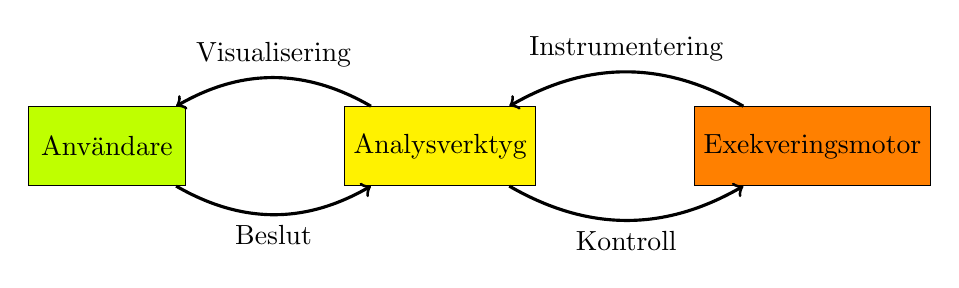
\begin{tikzpicture} \node [draw, fill=lime, minimum
	width=2cm, minimum height=1cm, ]  (user) {Användare};

		\node [draw, fill=yellow, minimum width=2cm, minimum height=1cm,
		right=2cm of user ] (tool) {Analysverktyg};

		\node [draw, fill=orange, minimum width=2cm, minimum height=1cm,
		right=2cm of tool ] (engine) {Exekveringsmotor};

		\draw[->, line width=.4mm] (user.-30) to[out=-30, in=-150]
		node[midway,below]{Beslut} (tool.-150);

		\draw[->, line width=.4mm] (tool.150) to[out=150, in=30]
		node[midway,above]{Visualisering} (user.30);

		\draw[->, line width=.4mm] (tool.-30) to[out=-30, in=-150]
		node[midway,below]{Kontroll} (engine.-150);

		\draw[->, line width=.4mm] (engine.150) to[out=150, in=30]
		node[midway,above]{Instrumentering} (tool.30);

	\end{tikzpicture} \caption{ Schematisk bild av ett binäranalysverktyg byggt
	kring en exekveringsmotor }\label{schematic} \end{figure}

\subsubsection{Analyser}

Det finns många möjliga analyser som kan användas av ett binäranalysverktyg, där
\textit{analyser} avser en visualisering av en aspekt av det analyserade
programmets beteende eventuellt inklusive ett sätt för användaren att påverka
det analyserade programmets körning.

En konkret exekvering kan spåras och dess instruktionssekvens kan visas för
användaren med loopar identifierade. Flera exekveringar kan visualiseras på
samma sätt och deras instruktionssekvenser användas för att återskapa
kontrollflödesstrukturer som for- och while-loopar och if-satser.

Möjligheter för \textit{state merging} kan identifieras helautomatiskt eller av
användaren, alltså platser där flera exekveringar kan ersättas av en enda mer
generell exekvering som innehåller ursprungsexekveringarnas skillnader som
symboliska uttryck.

En uppsättning liknande exekveringar kan visas upp för användaren tillsammans
med information om när och hur de divergerar, för att till exempel avgöra när
olika delar av indatan används.

För analys av programmet är det också hjälpsamt för användaren att kunna stega
genom exekveringen steg för steg och ändra på värden för att ta de vägar de vill
analysera. Detta borde också kunna göras baklänges, det vill säga att användaren
väljer en slutdestination och låter programmet själv lista ut vilka värden som
behövdes läsas för att exekveringen skulle ta sig till den punkten.

En mer automatisk men ändå viktig funktionalitet är konstruktion av kod-täckande
indata. När testfall som besöker en uppsättning instruktioner är konstruerad kan
kraven på indatan över denna uppsättning programhopp analyseras och programmet
kan lista ut vilka aspekter av indatan som kan ändras utan att påverka
kodtäckningsgraden, och kommunicera detta till användaren.

Det finns många möjliga analyser. Användbarheten i ett verktyg mäts inte i
kvantiteten analyser utan i förmågan för de utvalda implementerade analyserna
att täcka användarens behov av förståelse av programmet.


I avsikt att utveckla ett binäranalysverktyg, bestämdes det att ta fram demon
(demonstrationer) som ska leda det kontinuerliga utvecklingsarbetet.

Ett demo ska bestå av en analys med hjälp av verktyget som ökar förståelse för
ett exempelprogram. Med förståelse menas en abstrakt programförståelse
beskrivet i bakgrundsavsnittet. Exempelprogrammet ska framställas med en
egenskap som man skulle vilja kunna detektera med ett analysverktyg. Mer
konkret ska ett sådant exempelprogram inneha t.ex. minnessårbarhet, ett oväntad
krasch eller något annat sårbarhet som inte önskas i ett program.

Exempelprogrammen ska skrivas i C för enkelhetens skull eftersom C-programs
utseende i binärformat relativt väl motsvarar deras källkod. 

Sedan ska exempelprogrammet kompileras till en binär som analyseras med
analysverktyget med avsikt att detektera den kända egenskapen hos
exempelprogrammet. Om detta inte är möjligt med den nuvarande version av
analysverktyget ska analysverktyget utökas för att möjliggöra demot.

Detta tillvägagångssätt är önskvärt eftersom det tillåter att sätta uppnåbara
delmål som styr funktionalitet i analysverktyget som ska implementeras härnäst.
Dessutom kan flera demon utvecklas samtidigt vilket tillåter parallellism inom
utvecklingen och framsteg på flera fronter.

Tillvägagångssättet är jämförbart med den agila arbetsmetoden där utveckling sker 
evolutionärt. Detta är önskvärt då verktygets potentiella 
användningsbarhet inte är självklar på detaljnivå.

I ett senare och/eller parallellt steg ska ett grafiskt användargränssnitt
utvecklas som tillåter användaren att navigera programmet som analyseras och
göra egna beslut gällande förgreningar etc. där användaren själv bestämmer
interaktivt nästa beslut som görs. Även detta arbete styrs av demon som
framställs och funktionaliteter som önskas.

\subsection{Evaluering och jämförelse med andra verktyg}

För att det ska gå att testa verktygets förmåga och jämföra med andra
analysverktyg ska de demon som tas fram bestå av CGC-binärer som analyseras. I
det fall CGC-binären är för komplicerat ska den förenklas samtidigt som den
originala sårbarheten återfinns, eller delas in i flera demon, tills dess att
den kompletta CGC-binären kan analyseras och sårbarheten detekteras.

Samma CGC-binärer som kan analyseras med det framställda analysverktyget ska
analyseras med binäranalysverktygen \emph{Angr} och \emph{Ghidra} och
analysresultatet jämföras för att göra en kvalitativ evaluering av eventuella
för- och nackdelar med det framtagna analysverktyget jämfört med de ovan nämnda
existerande verktygen. Jämförelsen kommer att ta hänsyn till hur snabbt det
gick att genomföra analysen, hur mycket ansträngning det krävde från
användaren, om det överhuvudtaget gick att hitta sårbarheten i CGC-binären, och
eventuellt andra för och nackdelar.

Val av CGC-binärer att analysera kommer att vara slumpmässigt med undantag för
fall då det anses ta för långt tid att utveckla vårt verktyg för att tillåta
analys av programmet med hänsyn till tidsbegränsningen för detta projekt.



\section{AMBA}


\section{Resultat}

\section{Diskussion}


\chapter{Slutsats}


\printbibliography

\end{document}
